% 0521(본책 94쪽) — 원에 내접하는 □ABCD 와 대각선 AC, ∠BAD=60°, 호 AB=호 AD 표시, BC=3cm·CD=2cm 파선 호. 답(AC)은 적지 않는다. 다시 그림.
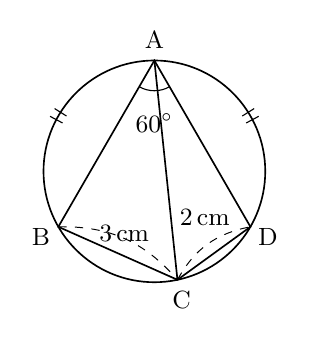
\begin{tikzpicture}[scale=1.28, line width=0.6pt]
  \draw (0.000,0.000) circle (1.100);
  \draw (0.000,1.100) -- (-0.953,-0.550) -- (0.229,-1.076) -- (0.953,-0.550) -- cycle;
  \draw (0.000,1.100) -- (0.229,-1.076);
  \draw[line width=0.4pt] (-0.150,0.840) arc[start angle=-120.000, end angle=-60.000, radius=0.300];
  \node[font=\small, inner sep=0.5pt] at (0.000,0.480) {$60^\circ$};
  \draw[line width=0.4pt] (-0.872,0.549) -- (-0.990,0.623);
  \draw[line width=0.4pt] (-0.911,0.480) -- (-1.035,0.546);
  \draw[line width=0.4pt] (0.911,0.480) -- (1.035,0.546);
  \draw[line width=0.4pt] (0.872,0.549) -- (0.990,0.623);
  \draw[dashed, line width=0.35pt] (-0.953,-0.550) to[bend left=25] (0.229,-1.076);
  \node[font=\small, inner sep=0.5pt] at (-0.300,-0.620) {$3\,\mathrm{cm}$};
  \draw[dashed, line width=0.35pt] (0.229,-1.076) to[bend left=25] (0.953,-0.550);
  \node[font=\small, inner sep=0.5pt] at (0.500,-0.460) {$2\,\mathrm{cm}$};
  \node[font=\small, inner sep=1.5pt] at (0.000,1.300) {A};
  \node[font=\small, inner sep=1.5pt] at (-1.126,-0.650) {B};
  \node[font=\small, inner sep=1.5pt] at (0.270,-1.272) {C};
  \node[font=\small, inner sep=1.5pt] at (1.126,-0.650) {D};
\end{tikzpicture}
